% Reconstruction test: boards 24 + 25 from CSEN 19 lecture, 06/05/2026.
% Source: board-extractor/output/csen19-v2/board-24_0h43m45s.png (t=43:45)
%         board-extractor/output/csen19-v2/board-25_0h25m55s.png (t=25:55)
% Style modeled on "Lecture 26 - Trees and Spanning Trees.pdf".
\documentclass[11pt]{article}
\usepackage[margin=1in]{geometry}
\usepackage{amsmath,amssymb,amsthm}
\usepackage{tikz}
\usetikzlibrary{positioning}

\newtheorem{theorem}{Theorem}
\theoremstyle{definition}
\newtheorem*{definition*}{Definition}

\title{CSEN 19: Characterizations of Trees and Spanning Trees}
\date{Lecture of June 5, 2026 \\ \small (reconstructed from boards at 25:55 and 43:45)}
\author{}

\begin{document}
\maketitle

\noindent
An acyclic graph is also called a \emph{forest}.
%
\begin{center}
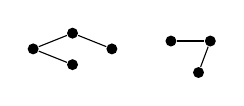
\begin{tikzpicture}[scale=0.5, every node/.style={circle, fill, inner sep=1.4pt}]
  % a small forest: two trees
  \node (a1) at (0,1) {};   \node (a2) at (1,1.4) {};
  \node (a3) at (1,0.6) {}; \node (a4) at (2,1) {};
  \draw (a2)--(a1)--(a3); \draw (a2)--(a4);
  \node (b1) at (3.5,1.2) {}; \node (b2) at (4.5,1.2) {};
  \node (b3) at (4.2,0.4) {};
  \draw (b1)--(b2); \draw (b2)--(b3);
\end{tikzpicture}
\end{center}

We continue proving the equivalence of the three characterizations of trees.
Recall the fact used for $(1)\Rightarrow(2)$: a tree must have a leaf (an
endpoint of a longest path); remove the leaf and apply induction to show that
a tree has exactly $m = n-1$ edges.

\paragraph{$(2)\Rightarrow(3)$.}
Assume $G$ is connected and $m = n-1$. \emph{Goal:} show $G$ is acyclic.

\begin{proof}
Suppose, to the contrary, that $G$ has a cycle. Remove an edge $e$ from the
cycle: the graph stays connected. Continue breaking cycles (one at a time)
until we get a connected and acyclic graph $\widetilde{G}$. Suppose we removed
in total $k$ edges ($k \ge 1$) to go from $G$ to $\widetilde{G}$.
Note: $\widetilde{G}$ is a tree!

Since $\widetilde{G}$ is a tree and
$|V(\widetilde{G})| = |V(G)| = n$, the graph $\widetilde{G}$ has exactly
$n-1$ edges. Also, $\widetilde{G}$ has $|E(G)| - k = n - 1 - k$ edges.
\[
  \therefore\quad n-1 \;=\; n-1-k \;\Longrightarrow\; k = 0,
  \quad \text{\underline{a contradiction}}.
\]
\end{proof}

\paragraph{$(3)\Rightarrow(1)$.}
Assume $G$ is acyclic and $m = n-1$. \emph{Goal:} show $G$ is connected.

\begin{proof}
Let $G$ have $c$ connected components. Then $G$ consists of a union of $c$
trees $T_1, T_2, \dots, T_c$. Hence
\[
  n-1 \;=\; m \;=\; |E(G)|
  \;=\; \sum_{i=1}^{c} |E(T_i)|
  \;=\; \sum_{i=1}^{c} \bigl(|V(T_i)| - 1\bigr)
  \;=\; \sum_{i=1}^{c} |V(T_i)| \;-\; \sum_{i=1}^{c} 1
  \;=\; n - c .
\]
\[
  \Longrightarrow\quad n-1 = n-c \quad\Longrightarrow\quad \boxed{c = 1}
\]
so $G$ must be connected.
\end{proof}

\bigskip

\begin{definition*}
Let $G$ be a connected graph. A \underline{spanning tree} of $G$ is a tree
$T \subseteq G$ ($T$ is a subgraph) such that $V(T) = V(G)$.
\end{definition*}

\begin{center}
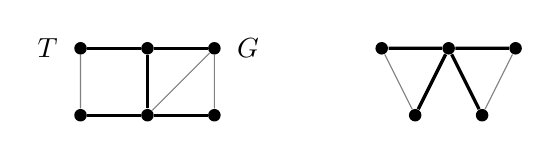
\begin{tikzpicture}[scale=0.85, every node/.style={circle, fill, inner sep=1.6pt}]
  % left: graph G with spanning tree T (tree edges thick)
  \node (v1) at (0,1) {}; \node (v2) at (1,1) {}; \node (v3) at (2,1) {};
  \node (v4) at (0,0) {}; \node (v5) at (1,0) {}; \node (v6) at (2,0) {};
  % non-tree edges of G (thin)
  \draw[gray, thin] (v1)--(v4) (v2)--(v5) (v3)--(v5) (v3)--(v6);
  % spanning tree T (thick)
  \draw[very thick] (v1)--(v2)--(v3) (v4)--(v5)--(v6) (v2)--(v5);
  \node[draw=none, fill=none, left=2pt of v1] {$T$};
  \node[draw=none, fill=none, right=2pt of v3] {$G$};

  % right: another graph with a spanning tree
  \begin{scope}[xshift=4.5cm]
    \node (w1) at (0,1) {}; \node (w2) at (1,1) {}; \node (w3) at (2,1) {};
    \node (w4) at (0.5,0) {}; \node (w5) at (1.5,0) {};
    \draw[gray, thin] (w1)--(w4) (w3)--(w5);
    \draw[very thick] (w1)--(w2)--(w3) (w2)--(w4) (w2)--(w5);
  \end{scope}
\end{tikzpicture}

\small (thick edges: one spanning tree)
\end{center}

\begin{theorem}
Every connected graph $G$ has a spanning tree.
\end{theorem}

\begin{proof}
Remove an edge from a cycle (repeatedly) until no more cycles exist. The
final subgraph is a spanning tree.
\end{proof}

\begin{theorem}
Let $G$ be a connected graph with $n \ge 2$ vertices. Then there exists a
vertex $v$ in $G$ such that $G - v$ is still connected.
\end{theorem}

\begin{proof}
Let $T$ be a spanning tree of $G$. Let $v$ be a leaf of $T$, that is,
$\deg_T(v) = 1$. Then $T - v$ is connected (because it is a tree), and
\[
  V(T-v) = V(G-v) \quad\text{and}\quad E(T-v) \subseteq E(G-v),
\]
so $G - v$ is connected as well.
\end{proof}

\end{document}
